\subsection{Clutter}
\label{sec:clutter}

We reproduce the clutter experiment from \cite{bib:castro2022unconstrained} to
evaluate solver performance in cluttered environments, common in robotic
manipulation. We drop 40 objects, arranged in four columns of 10, into an $80
\times 80 \times 80\text{ cm}$ box, see Fig. \ref{fig:clutter_initial_final}.
Each column has a mix of $10\text{ cm}$ diameter spheres and $10\text{ cm}$
boxes, with masses calculated using water density: $0.524\text{ kg}$ for spheres
and $1.0\text{ kg}$ for boxes. A high stiffness of $k=10^{7}\text{ N}/\text{m}$
models steel, with Hunt \& Crossley dissipation set to $d=10\text{ s}/\text{m}$
and SAP dissipation at $\tau_d=10^{-4} \text{ s}$. Lagged and Similar models use
a stiction tolerance of $v_s = 10^{-4}\text{ m}/\text{s}$, while SAP and the
regularized Lagged model use $\sigma=10^{-3}$. All surfaces have a friction
coefficient $\mu=1.0$. We let objects fall and simulate for $3$ seconds.

\begin{figure}[!h]
    \centering
    %trim={<left> <lower> <right> <upper>}
    \adjincludegraphics[height=0.65\columnwidth,trim={0 0 {0.05\width} 0},clip]{figures/TestCases/Clutter/initial_condition.png}
    \adjincludegraphics[height=0.65\columnwidth,trim={0 0 {0.05\width} 0},clip]{figures/TestCases/Clutter/final_condition.png}
    \caption{\label{fig:clutter_initial_final} Initial condition (left) and
    final steady state at $t=3$ seconds (right).}
\end{figure}

We analyze each method's performance with a time step $\delta
t=2\times10^{-3}\text{ s}$. Figure \ref{fig:clutter_iters_cn} shows Newton
solver iterations and Hessian condition numbers over time. An intense initial
transient occurs as objects collide upon falling, with impacts subsiding around
$t=2 \text{ s}$ as objects settle. During this early phase, the solver requires
more iterations, and condition numbers are higher. Notably, Lagged and Similar
approximations show higher condition numbers and iterations during the initial
transient, whereas the situation is reversed for SAP. This behavior relates to
the stiffness $G_t$ with regularized friction (Section
\ref{sec:impacts_and_conditioning}). Using the \emph{regularized} stiction
tolerance \eqref{eq:regularized_vs} in the Lagged approximation reduces
iterations and improves conditioning during the initial phase. Though not
included here, the same regularization can be used with Similar.

\begin{figure}[!h]
    \centering
    %trim={<left> <lower> <right> <upper>}
    \adjincludegraphics[height=0.375\columnwidth,trim={0 0 {0.05\width} 0},clip]{figures/TestCases/Clutter/SteelStiff/iterations_dt2em3.png}
    \adjincludegraphics[height=0.375\columnwidth,trim={0 0 {0.05\width} 0},clip]{figures/TestCases/Clutter/SteelStiff/condition_number_dt2em3.png}
    \caption{\label{fig:clutter_iters_cn} Iterations (left) and condition number
    (right) as a function of time. $\delta t=2\times10^{-3}\text{ s}$.}
\end{figure}

Figure \ref{fig:clutter_stiction_tolerance} shows the effective stiction
tolerance. For Lagged and Similar approximations, stiction tolerance is fixed at
$v_s=10^{-4}\text{ m}/\text{s}$ (dashed black line). In contrast, SAP and the
regularized Lagged approximation have a tolerance that varies with normal impulse
(Section \ref{sec:impacts_and_conditioning}). This aligns with prior
observations: during the initial transient, Lagged and Similar models enforce a
tighter friction approximation. Past this transient, SAP unnecessarily solves a
much tighter approximation.

\begin{figure}[!h]
    \centering
    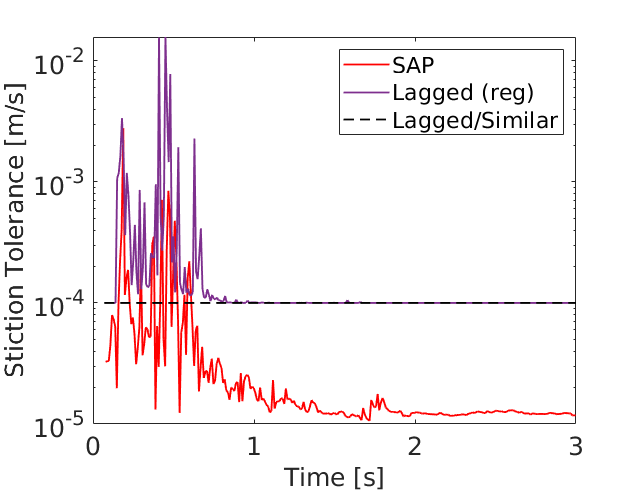
\includegraphics[width=0.8\columnwidth]{figures/TestCases/Clutter/SteelStiff/stiction_tolerance_dt2em3.png}
    \caption{Effective stiction tolerance as a function of time. $\delta t=2\times10^{-3}\text{ s}$.}
    \label{fig:clutter_stiction_tolerance}
\end{figure}

An informative metric is the mean iteration count and condition number as a
function of time step, Fig. \ref{fig:clutter_mean_iters_cn}. For SAP,
the condition number remains almost unchanged across time step sizes since
$G_t=1/R_t$ (see Section \ref{sec:impacts_and_conditioning}) is constant. In contrast,
the conditioning of Lagged and Similar models improves as the time step decreases,
because $G_t$ is proportional to impulse and time step size. This reduction explains
why the number of iterations decreases for Lagged and Similar as the time step
decreases, while for SAP, it remains almost constant. Figure
\ref{fig:clutter_mean_iters_cn} also highlights the benefit of regularization
for Lagged at large time steps. At small time steps, $v_s$ dominates in
\eqref{eq:regularized_vs}, making Lagged with and without regularization perform
similarly.

\begin{figure}[!h]
    \centering
    %trim={<left> <lower> <right> <upper>}
    \adjincludegraphics[height=0.375\columnwidth,trim={0 0 {0.05\width} 0},clip]{figures/TestCases/Clutter/SteelStiff/mean_iters.png}
    \adjincludegraphics[height=0.375\columnwidth,trim={0 0 {0.05\width} 0},clip]{figures/TestCases/Clutter/SteelStiff/mean_cn.png}
    \caption{\label{fig:clutter_mean_iters_cn} Mean number of iterations (left) and
    condition number (right) per time step as a function of time step size.}
\end{figure}


We examine compliance as a method for approximating \emph{rigid} contact by
measuring mean penetration distance over the last $1.25$ seconds, when objects
settle at the bottom of the box. Figure \ref{fig:clutter_penetration_study}
shows steady-state penetration across stiffness values spanning eight orders of
magnitude. For reference, Hertz theory predicts a stiffness of $10^7\text{
N}/\text{m}$ for steel. We stress-test with stiffness up to five orders higher,
confirming the robustness of the convex formulation. For a time step $\delta
t=0.005\text{ s}$, SAP’s \emph{near-rigid} \cite{bib:castro2022unconstrained}
stiffness estimate is $10^6\text{ N}/\text{m}$, with penetration at only tenths
of microns. At an extreme, nonphysical $k=10^{13}\text{ N}/\text{m}$, the solver
fails due to round-off errors, while $10^5-10^6\text{ N}/\text{m}$ suffices for
approximating rigid contact in typical robotics applications.

\begin{figure}[!h]
    \centering
    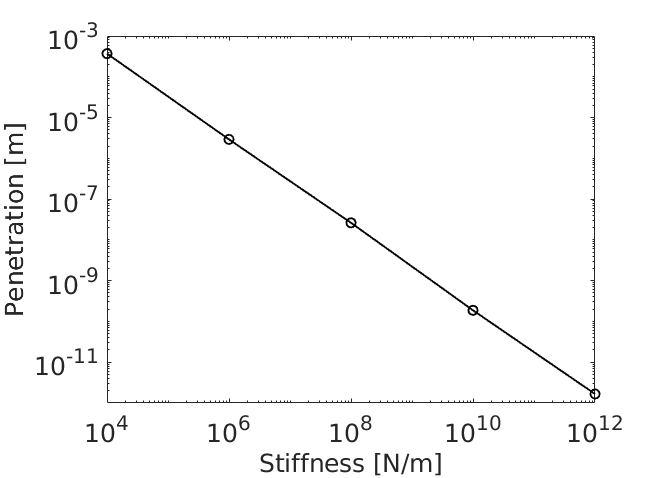
\includegraphics[width=0.8\columnwidth]{figures/TestCases/Clutter/StiffnessStudy/steady_state_penetration.png}
    \caption{Mean penetration distance in steady state during the last $1.25\text{ s}$
    of the simulation.}
    \label{fig:clutter_penetration_study}
\end{figure}

Finally, figure \ref{fig:clutter_stiffness_study} shows the effect of stiffness
on performance. As expected, higher stiffness values degrade conditioning and
ultimately impair performance. However, we note that the performance degradation
is minimal --- only within $20\%$, even for stiffness values as high as those of
steel.

\begin{figure}[!h]
    \centering
    %trim={<left> <lower> <right> <upper>}
    \adjincludegraphics[height=0.375\columnwidth,trim={0 0 {0.05\width} 0},clip]{figures/TestCases/Clutter/StiffnessStudy/iterations.png}
    \adjincludegraphics[height=0.375\columnwidth,trim={0 0 {0.05\width} 0},clip]{figures/TestCases/Clutter/StiffnessStudy/cond_number.png}
    \caption{\label{fig:clutter_stiffness_study} Mean number of iterations (left) and
    condition number (right) per time step as a function of stiffness.}
\end{figure}
